\documentclass[../poliXuniversity_hospital_-USP-report.tex]{subfiles}
\graphicspath{ {images/}{../images/}{../../images/} }
\begin{document}
\clearpage

\section{Interface com Usuário}

A placa de Interface com o usuário é uma das que deram mais problemas. Ela foi idealizada, desde da primeira versão do robô hospitalar, para realizar a leitura de cartões, para retirada de entregas do robô hospitalar, abertura e controle do motor das quatro portas do robô hospitalar, além, é claro, de enviar informações para o módulo de controle.

\subsection{Placa}

Como módulo, existem muitas minúcias que precisamos tomar ao projetá-las. A placa de Interface com o usuário, para segunda versão do robô hospitalar, com objetivo de evitar problemas e realizar testes, teve duas versões: um protótipo, que já foi finalizado, e uma versão oficial, ainda em desenvolvimento. 

%================================ INTERFACE COM USUARIO PROTÓTIPO ========================
\subsubsection{Protótipo}

O protótipo das placas foi refeito três vezes. Como se trata de uma placa fresada, pode ser refeita no próprio laboratório do professor orientador. A primeira placa não funcionou porque a impressão ficou ruim. O projeto da placa eletrônica, assim como o de todos os módulos, foi dividido em esquemático e Printed Circuit board (PCB) . 

\begin{figure}[!ht]
\centering
    \caption{Protótipo placa de Interface com Usuário - Esquemático principal }
    \centering % para centralizarmos a figura
    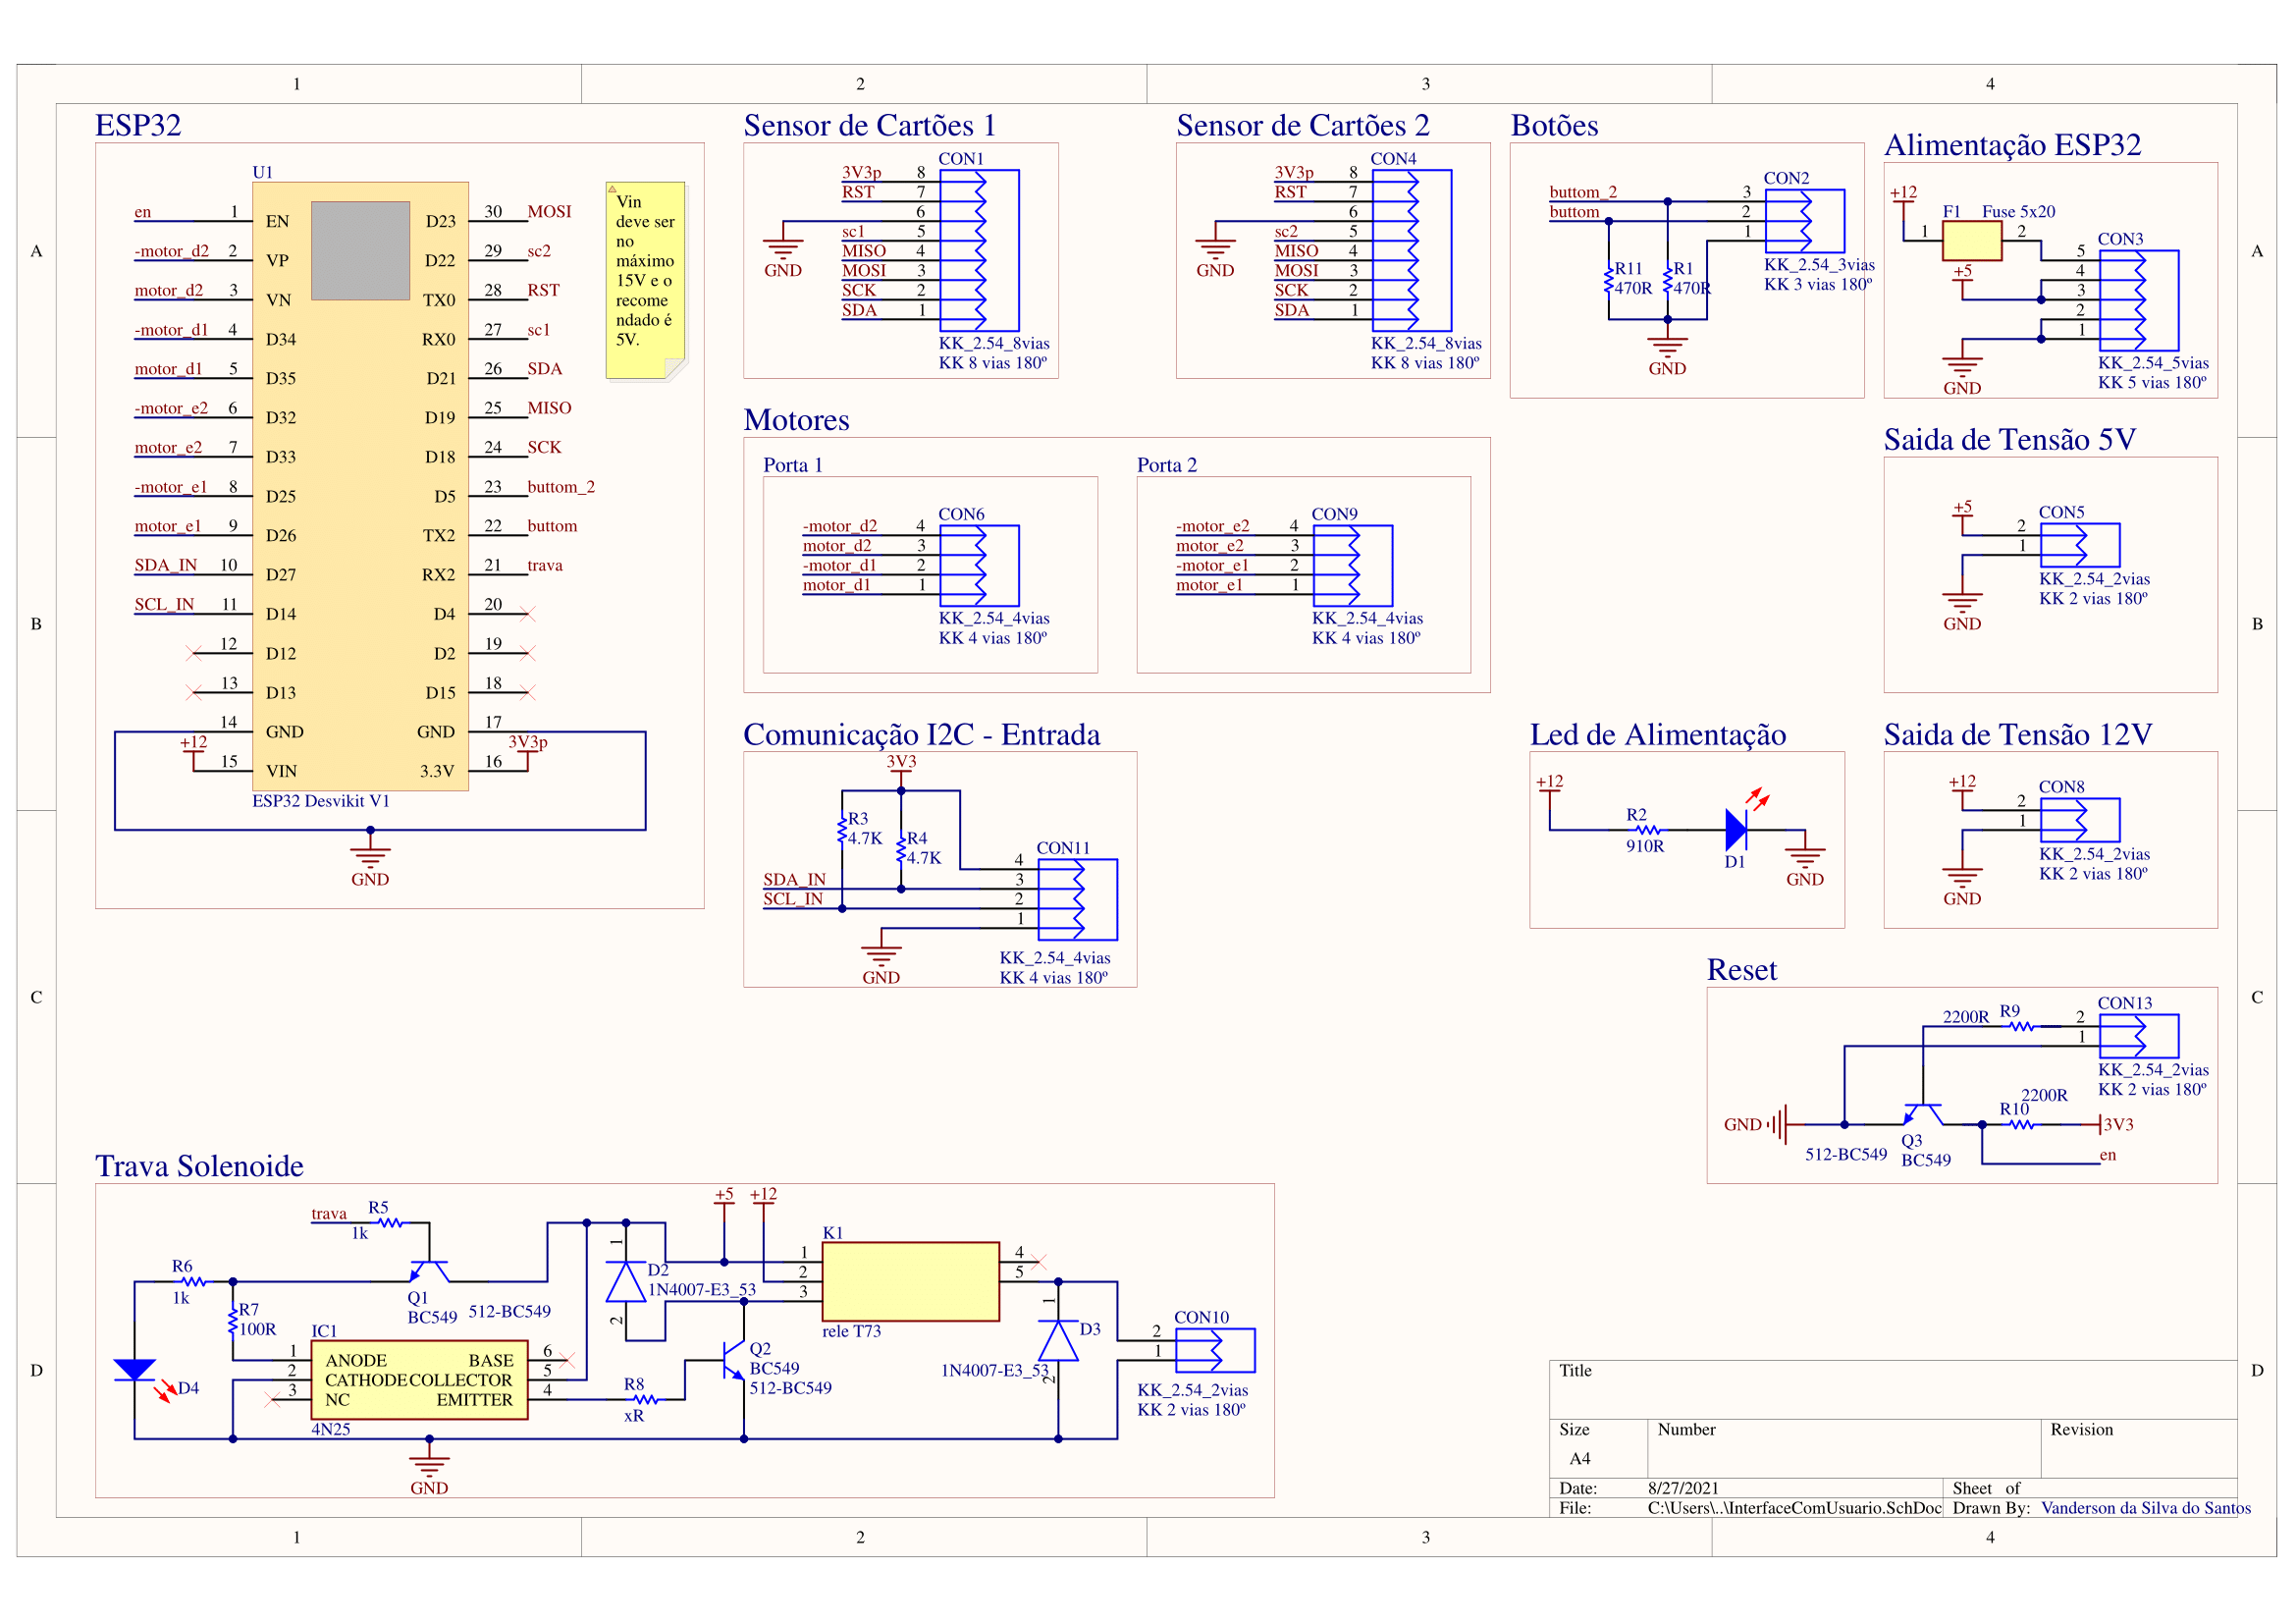
\includegraphics[width=15cm]{modulos/InterfaceComUsuario-1.png}
    \caption*{Fonte: Elaborado pelo autor no software Altium Design\cite{altium21} }
    \label{Protótipo placa de ## - Esquemático principal}
\end{figure}

Para design do hardware do módulo de Interface com Usuário foi utilizado o CAD e software Altium Designer 21 \cite{altium21} a partir de uma licença estudantil. O projeto completo está disponibilizado em \cite{github_modulos} e todos os componentes usado nesse protótipo podem ser visto na tabela ~\ref{table:Componentes Utilizados na placa de Interface com Usuário - Protótipo}.

\begin{table}[!ht]
\caption{Componentes Utilizados na placa de Interface com Usuário - Protótipo}
\centering
\begin{adjustbox}{width=\columnwidth,center}
\begin{tabular}{|c|c|c|c|c|}
\hline
Component                   & Description                                    & Designator                             & Footprint                   & Quantity \\ \hline
KK\_2.54\_8vias             & Conector KK 2.54mm 8   vias                    & CON1, CON4                             & KK\_8vias\_180°             & 2        \\ \hline
KK\_2.54\_3vias             & Conector KK 2.54mm 3   vias                    & CON2                                   & KK\_3vias\_180º             & 1        \\ \hline
KK\_2.54\_5vias             & Conector KK 2.54mm 5   vias                    & CON3                                   & KK\_5vias\_180°             & 1        \\ \hline
KK\_2.54\_2vias             & Conector KK 2.54mm 2   vias                    & CON5, CON8, CON10,   CON13             & KK\_2VIAS\_180º             & 4        \\ \hline
KK\_2.54\_4vias             & Conector KK 2.54mm 4   vias                    & CON6, CON9, CON11                      & KK\_4vias\_180°             & 3        \\ \hline
LED 5MM RED                 & LED 5MM RED                                    & D1, D4                                 & LED 5MM RED                 & 2        \\ \hline
1N4007-E3\_53               & Diode                                          & D2, D3                                 & DIOAD1405W89L465D235        & 2        \\ \hline
Fuse 5x20                   & Fuse                                           & F1                                     & Fuse 5x20                   & 1        \\ \hline
4N25                        & Integrated Circuit                             & IC1                                    & DIP762W50P254L712H450Q6N    & 1        \\ \hline
rele T73                    & Relay or Contactor                             & K1                                     & JQC3FT731Z12VDC             & 1        \\ \hline
BC549                       & TRANS NPN 30V 0.1A   TO-92                     & Q1, Q2, Q3                             & TO92                        & 3        \\ \hline
RES 470R 1/4W   CARBON FILM & RES 470R OHM 1/4W 5\%   CARBON FILM            & R1, R2, R5, R6, R7,   R8, R9, R10, R11 & RES 470R 1/4W CARBON   FILM & 9        \\ \hline
4.7K                        & RES 4.7K OHM 1/4W 5\%   CARBON FILM            & R3, R4                                 & RES 4.7K 1/4W CARBON   FILM & 2        \\ \hline
microcontrolador            & microcontrolador com   moculo bluethoth e wifi & U1                                     & ESP32\_Desvikit\_v1         & 1        \\ \hline

\end{tabular}
\end{adjustbox}
\centering
\caption*{Fonte: Elaborado pelo autor}
\label{table:Componentes Utilizados na placa de Interface com Usuário - Protótipo}
\end{table}

Dentre os componentes usados, destaca-se o rele T73 \cite{rele_T73_datasheet} e o optoacoplador 4N25 \cite{4N25_datasheet} , utilizado nas solenoides da porta. Além disso, como já mencionado antes, também usamos o ESP32 \cite{esp32} como microcontrolador do módulo.

A partir do esquema elétrico que foi feito e do desenho da PCB, a placa de circuito impresso, em uma única camada (Single Layer) e dimensões de 120x60mm. As visões 2D e 3D podem ser vista na figura ~\ref{Protótipo Interface com Usuário - PCB 2D} e ~\ref{Protótipo Interface com Usuário - PCB 3D}.

\begin{figure}[!ht]
    \centering
    \begin{minipage}{0.5\textwidth}
        \centering
        \caption{Protótipo Interface com Usuário - PCB 2D}
        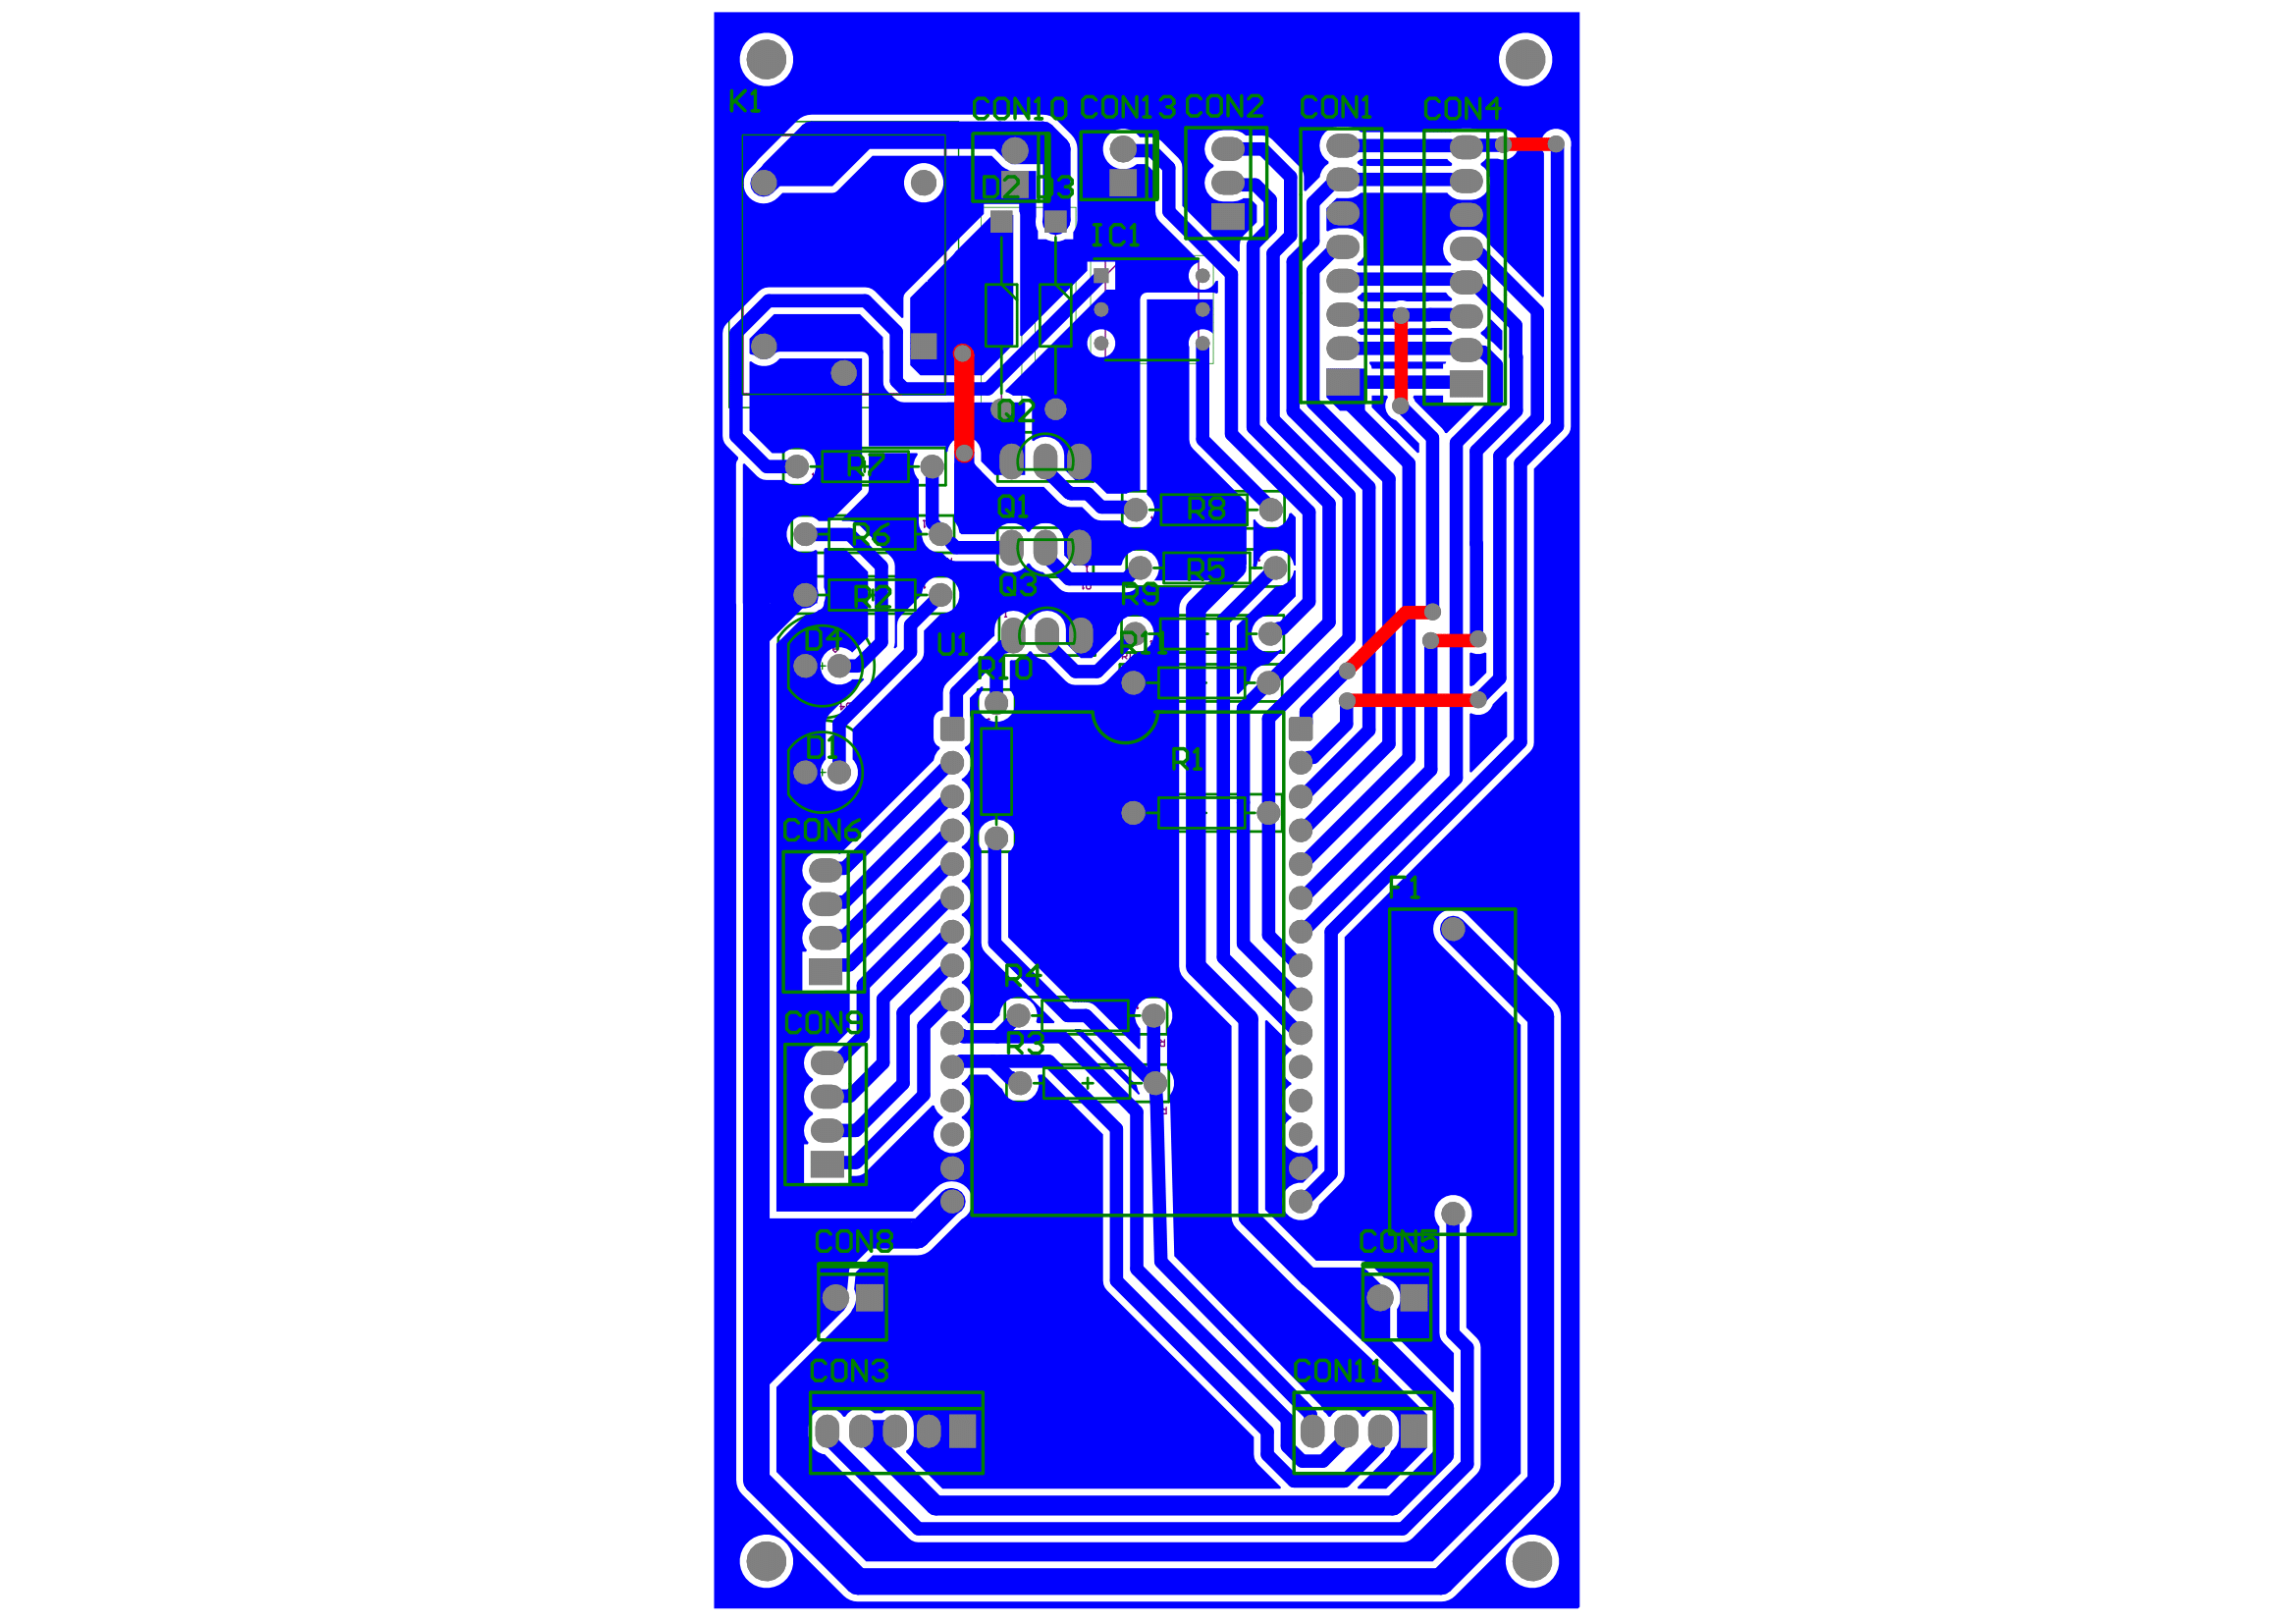
\includegraphics[width=1.03\textwidth]{modulos/InterfaceComUsuario-2.png} 
        \label{Protótipo Interface com Usuário - PCB 2D}
    \end{minipage}\hfill
    \begin{minipage}{0.5\textwidth}
        \centering
        \caption{Protótipo Interface com Usuário - PCB 3D }
        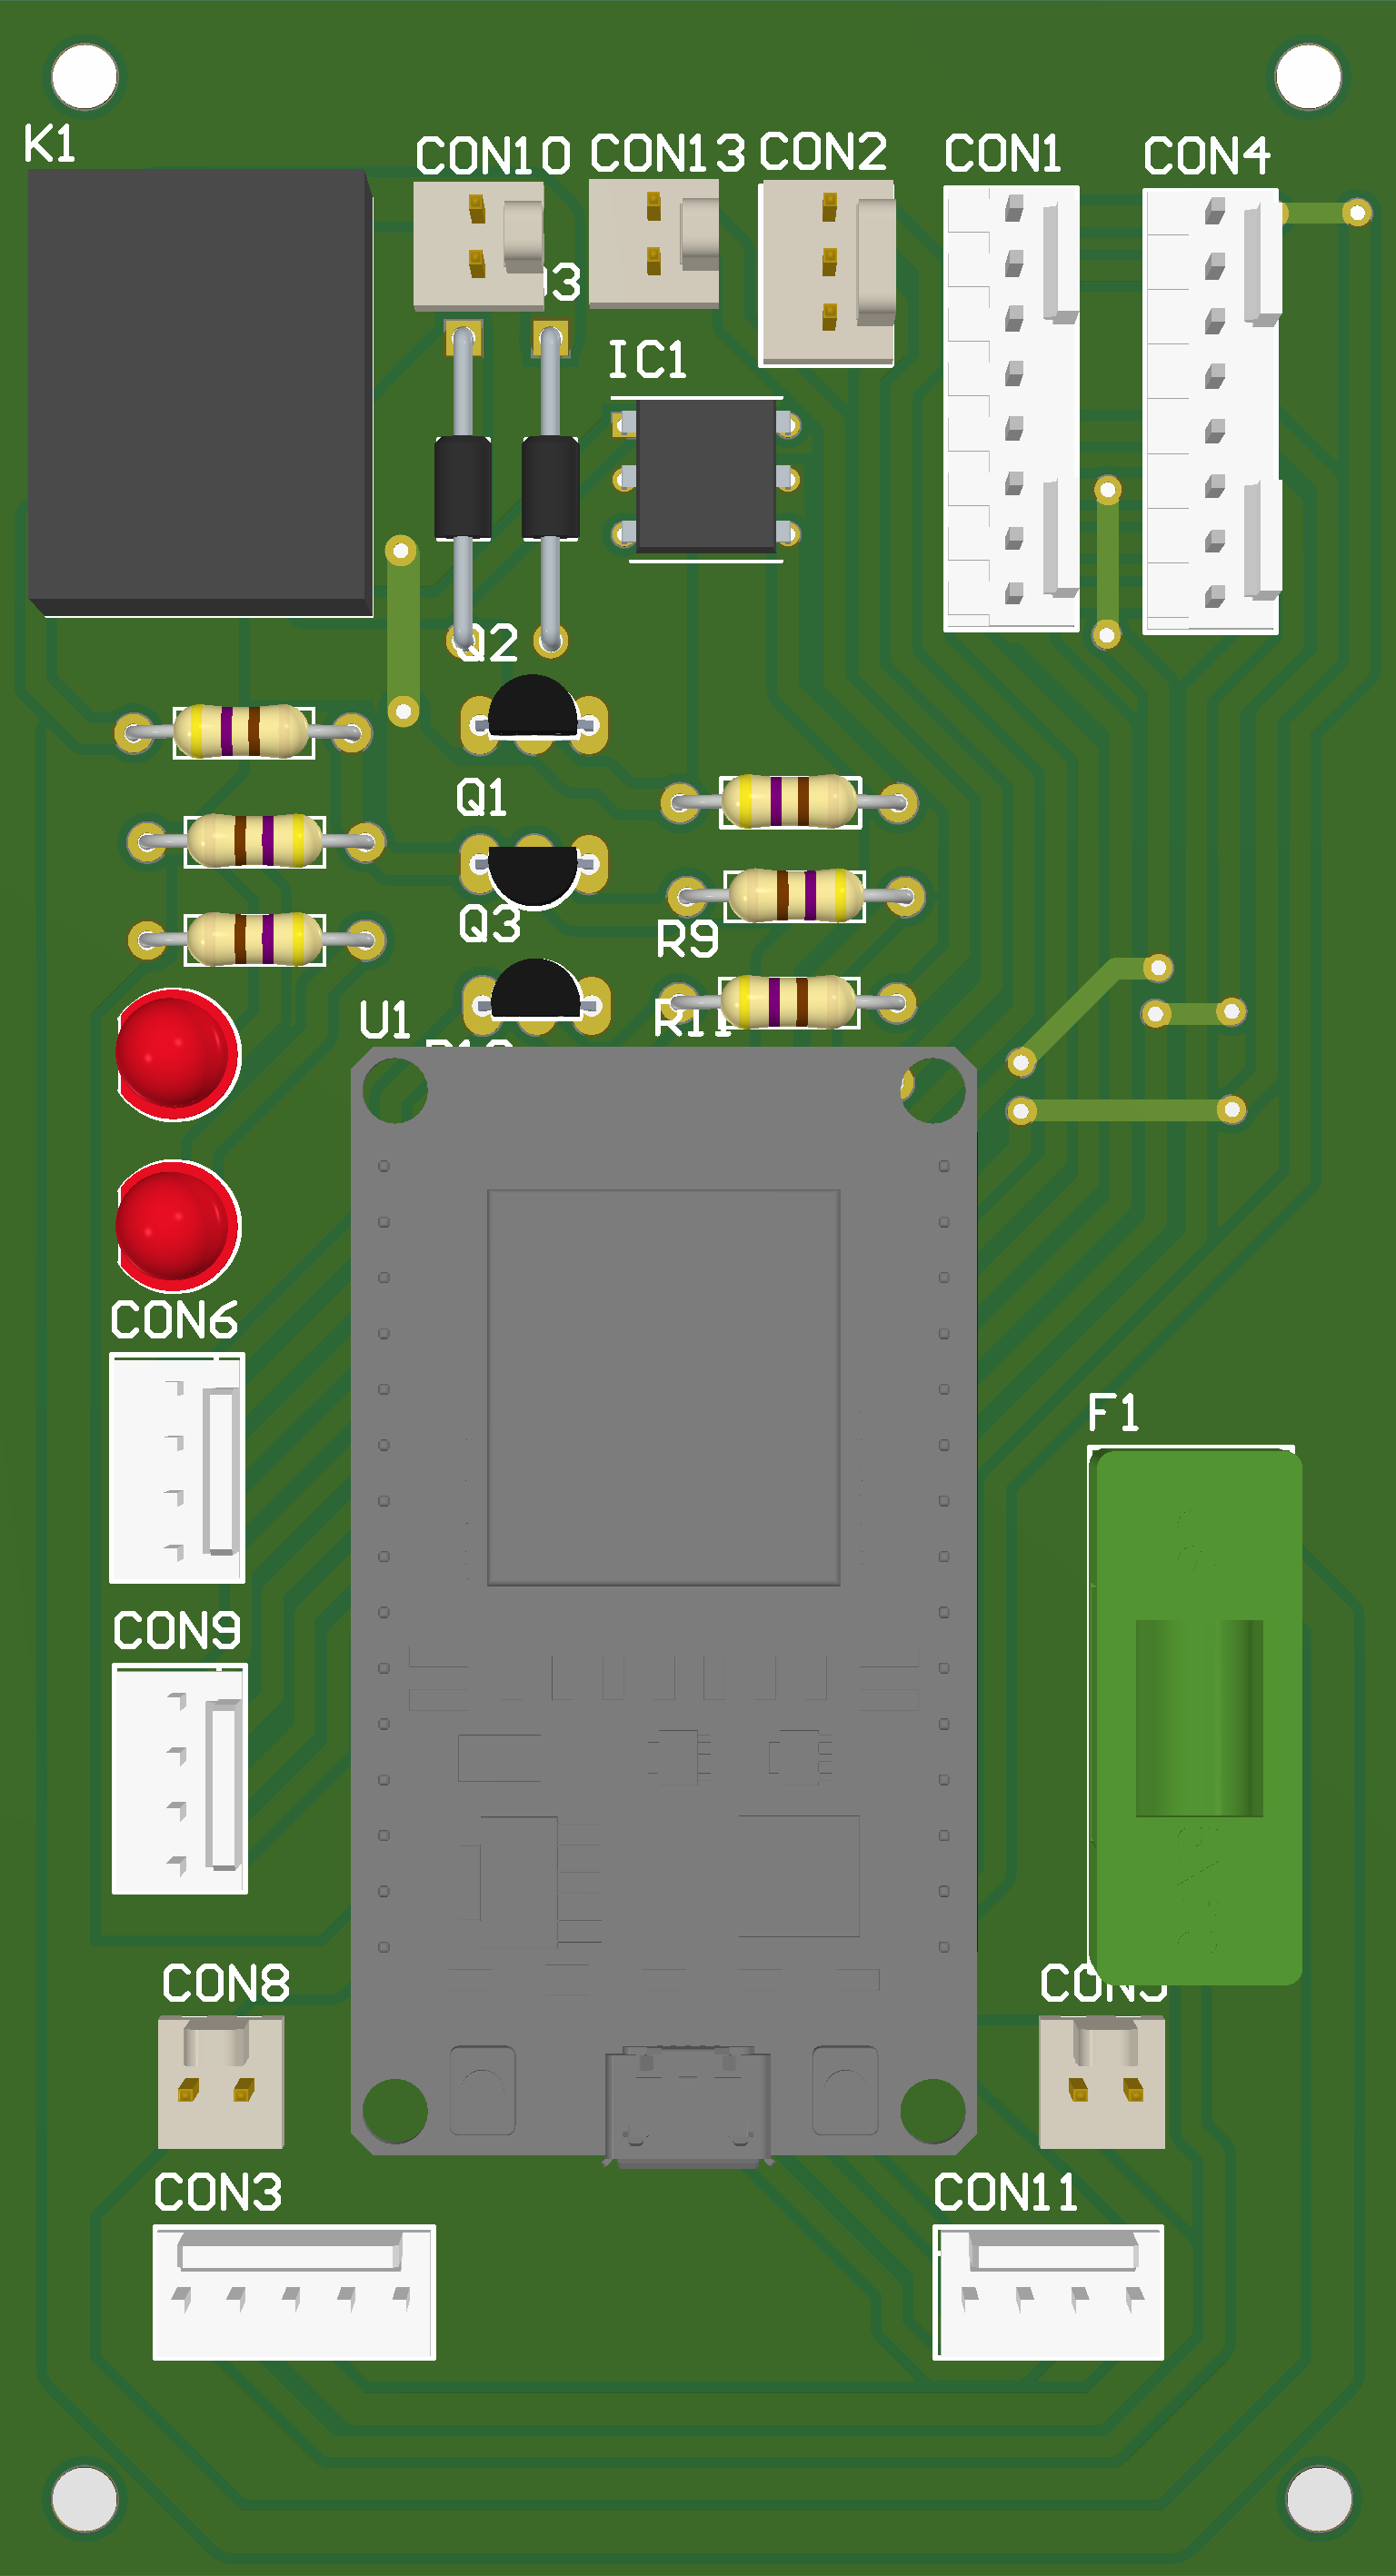
\includegraphics[width=0.4\textwidth]{modulos/InterfaceComUsuario.png} 
        \label{Protótipo Interface com Usuário - PCB 3D}
    \end{minipage}\hfill
    
    \caption*{Fonte: Elaborado pelo autor no software Altium Design\cite{altium21} }
    \label{fig:Protótipo Interface com Usuário - PCB 2D3D}
\end{figure}

\begin{comment}
\begin{figure}[!ht]
    \centering
    \begin{minipage}{0.5\textwidth}
        \centering
        \caption{Protótipo Interface com Usuário - Trilhas}
        \includegraphics[width=0.8\textwidth]{example-image-a} 
        \label{fig:figura1minipg}
    \end{minipage}\hfill
    \begin{minipage}{0.5\textwidth}
        \centering
        \caption{Protótipo Interface com Usuário - Completa }
        \includegraphics[width=0.8\textwidth]{example-image-a} 
        \label{fig:figura1minipg}
    \end{minipage}\hfill
    \caption*{Fonte: Elaborado pelo autor }
    \label{fig:Protótipo Interface com Usuário - TrilhasC}
\end{figure}
\end{comment}
%================================ INTERFACE COM USUARIO OFICIAL ========================
\clearpage
\subsubsection{Oficial}

A placa oficial de Interface com o usuário ainda não foi fabricada. Por se tratar de uma placa mais profissional, ela será mandada para ser feita para uma empresa privada ainda não escolhida, não na própria Universidade São Paulo. Assim como o protótipo, o projeto como um todo foi dividido em um esquemático e uma PCB.

\begin{figure}[!ht]
\centering
    \caption{placa de Interface com Usuário - Esquemático principal }
    \centering % para centralizarmos a figura
    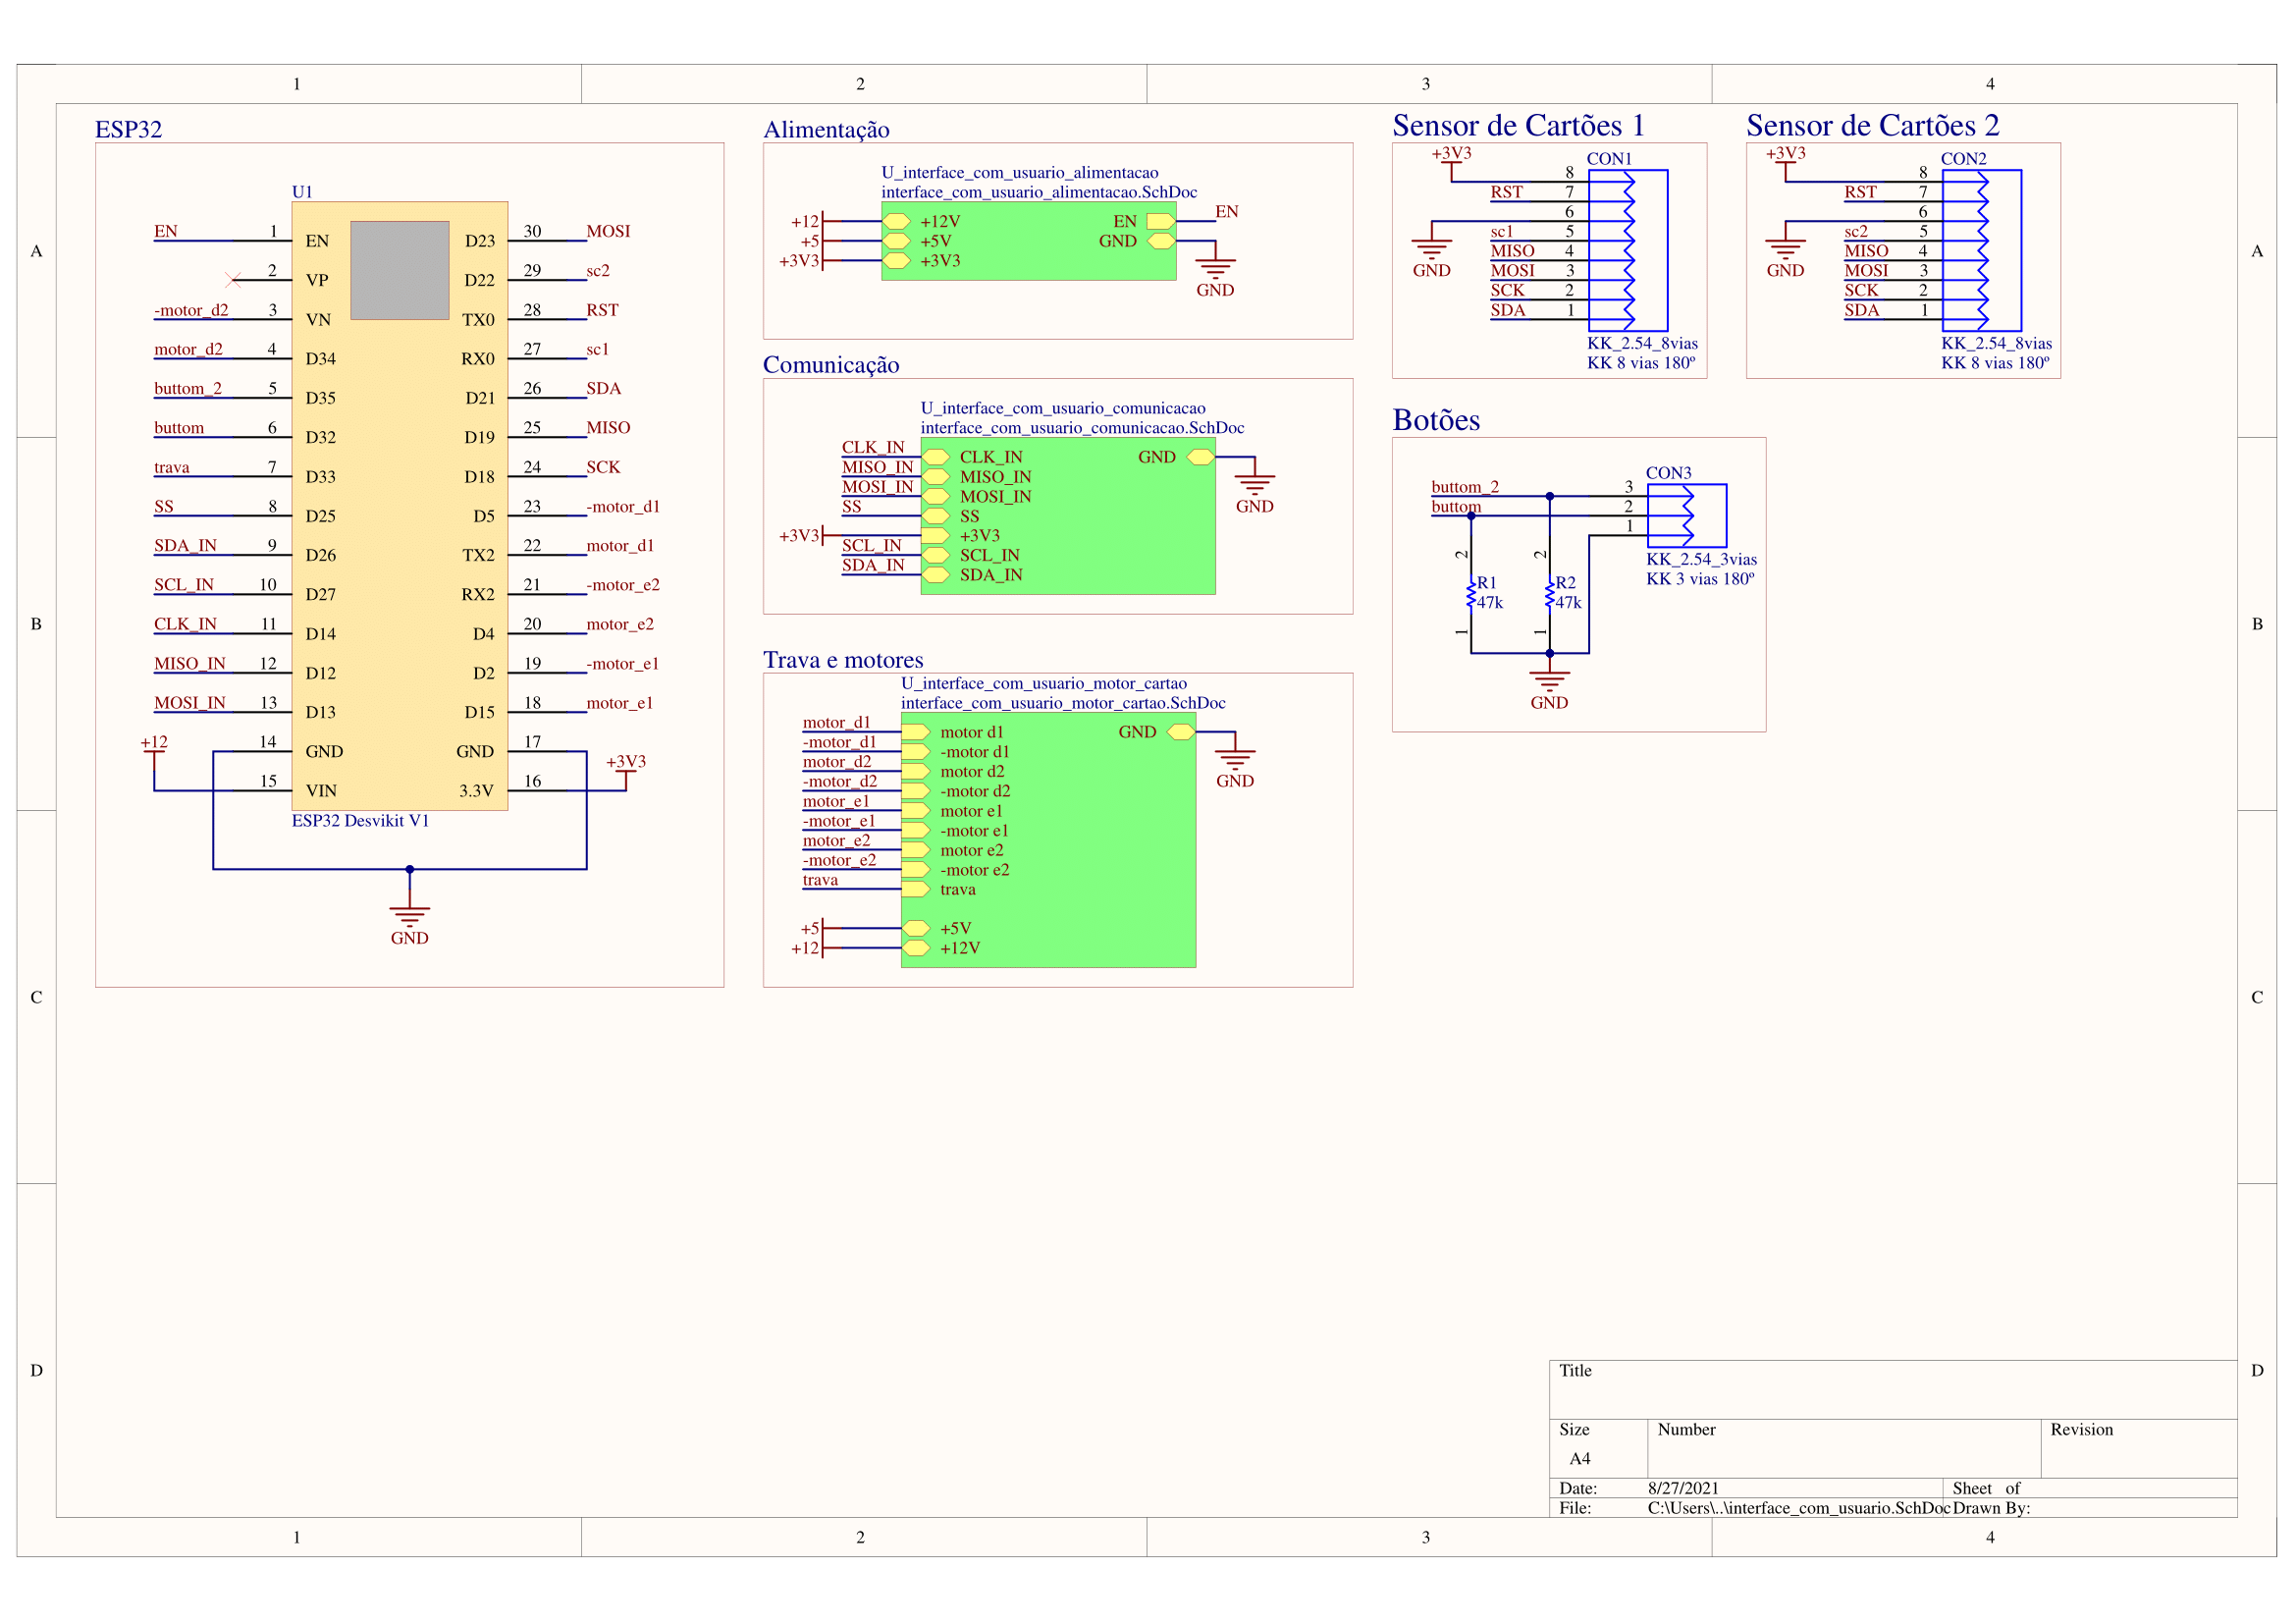
\includegraphics[width=17cm]{modulos/interface_com_usuario-1.png}
    \caption*{Fonte: Elaborado pelo autor no software Altium Design\cite{altium21} }
    \label{Protótipo placa de ## - Esquemático principal}
\end{figure}

Para design do hardware do módulo de Interface com o usuário foi utilizado o CAD e software Altium Designer 21 \cite{altium21} a partir de uma licença estudantil. O projeto completo está disponibilizado em \cite{github_modulos} e todos os componentes usado nessa versão oficial podem ser visto na tabela ~\ref{table:Componentes Utilizados na placa de Interface com Usuário}.

\begin{table}[!ht]
\caption{Componentes Utilizados na placa de Interface com Usuário}
\centering
\begin{adjustbox}{width=\columnwidth,center}
\begin{tabular}{|c|c|c|c|c|}

\hline
Component        & Description                                    & Designator                                                           & Footprint           & Quantity \\ \hline
KK\_2.54\_8vias  & Conector KK 2.54mm 8   vias                    & CON1, CON2                                                           & KK\_8vias\_180°     & 2        \\ \hline
KK\_2.54\_3vias  & Conector KK 2.54mm 3   vias                    & CON3                                                                 & KK\_3vias\_180º     & 1        \\ \hline
KK\_2.54\_2vias  & Conector KK 2.54mm 2   vias                    & \begin{tabular}[c]{@{}l@{}}CON4, CON6, \\ CON7,   CON12\end{tabular} & KK\_2VIAS\_180º     & 4        \\ \hline
KK\_2.54\_6vias  & Conector KK 2.54mm 6   vias                    & CON5                                                                 & KK\_6vias\_180°     & 1        \\ \hline
KK\_2.54\_5vias  & Conector KK 2.54mm 5   vias                    & CON8                                                                 & KK\_5vias\_180°     & 1        \\ \hline
KK\_2.54\_4vias  & Conector KK 2.54mm 4   vias                    & CON9, CON10, CON11                                                   & KK\_4vias\_180°     & 3        \\ \hline
LED 3MM RED      & LED 3MM RED                                    & D1                                                                   & LED RED             & 1        \\ \hline
1N4007 smd       & Diode smd                                      & D2, D3                                                               & DIOM5327X242N       & 2        \\ \hline
rele T73         & Relay or Contactor                             & K1                                                                   & JQC3FT731Z12VDC     & 1        \\ \hline
Trans BC817      & Transistor BJT NPN   BC817-25-7-F              & Q1, Q2, Q4                                                           & SOT96P240X110-3N    & 3        \\ \hline
4N25-X007T       & Phototransistor                                & Q3                                                                   & SOP254P1030X440-6N  & 1        \\ \hline
47k              & RES 1206 5\%                                   & R1, R2                                                               & RESC3216X60N        & 2        \\ \hline
680R             & Resistor                                       & R3                                                                   & RESC3216X60N        & 1        \\ \hline
2k2              & Resistor                                       & R4, R5                                                               & RESC3216X60N        & 2        \\ \hline
4k7              & RES 1206 5\%                                   & R6, R7                                                               & RESC3216X60N        & 2        \\ \hline
1k               & RES 1206 5\%                                   & R8, R10                                                              & RESC3216X60N        & 2        \\ \hline
100R             & RES 1206 5\%                                   & R9                                                                   & RESC3216X60N        & 1        \\ \hline
microcontrolador & microcontrolador com   moculo bluethoth e wifi & U1                                                                   & ESP32\_Desvikit\_v1 & 1        \\ \hline

\end{tabular}
\end{adjustbox}
\centering
\caption*{Fonte: Elaborado pelo autor}
\label{table:Componentes Utilizados na placa de Interface com Usuário}
\end{table}

Em relação ao protótipo, pouco mudou da lógica por trás do circuito, a principal diferença é que o modelo oficial utiliza todos componentes com encapsulamiento SMD \cite{SMD_def}. Além disso, foi adicionado o protocolo de comunicação SPI também, como já foi comentado no início do capítulo.


A placa de circuito impresso ainda está em desenvolvimento.

\begin{comment}
%================================ INTERFACE COM USUARIO FIRMWARE ========================
\subsection{Firmware}
\end{comment}

\end{document}